\begin{ledgroupsized}[r]{120mm}
\footnotesize
\pstart
\noindent\textbf{\"{U}berlieferung:}
\pend
\end{ledgroupsized}
%
\begin{ledgroupsized}[r]{114mm}
\footnotesize
\pstart \parindent -6mm
\makebox[6mm][l]{\textit{L}}%
Reinschrift mit Ergänzungen und 
Verbesserungen: LH XXXVII 3 Bl. 162-163. 1 Bog. 2\textsuperscript{o}.
1\,\unitfrac{1}{4} S. auf Bl.~162~r\textsuperscript{o} und 163~v\textsuperscript{o}, zweispaltig.
Bl.~162~v\textsuperscript{o} und 163~r\textsuperscript{o} sind leer.
Wasserzeichen auf Bl.~162. Am oberen Rand von Bl. 163~r\textsuperscript{o} gestrichenes Wort \textit{Quae}.
\\%
Cc 2, Nr. 480 A-B
\pend
\end{ledgroupsized}
%
\vspace*{5mm}
\begin{ledgroup}
\footnotesize
\pstart
\noindent\footnotesize{\textbf{Datierungsgr\"{u}nde}:
Anhand des Wasserzeichens lässt sich das vorliegende Stück auf den Zeitraum von Juni 1672 bis März 1673 datieren.}
\pend
\end{ledgroup}
%
\vspace*{8mm}
\count\Afootins=1200
\count\Bfootins=1000
\count\Cfootins=1200
%\begin{center}
%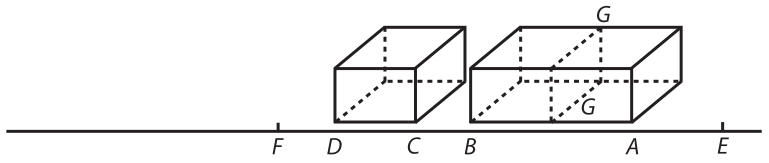
\includegraphics[width=0.85\textwidth]{images/lh03703_162r-d1.pdf}\\
%\rule[0pt]{0pt}{0pt}[\textit{Fig. 1}]
%\end{center}
\pstart%
\normalsize%
\noindent%
[162~r\textsuperscript{o}] \edtext{In vacuo\protect\index{Sachverzeichnis}{vacuum}, seu quod idem est, corporibus per se consideratis, nihil refert quanta sit corporum concurrentium longitudo, seu si}{\lemma{}\Bfootnote{\textit{(1)} Si duo corpora \textbar\ cylindrica\protect\index{Sachverzeichnis}{corpora cylindrica} aeque lata, inter se inaequaliter longa \textit{erg.} \textbar\ sibi directe occurrant basibus integris, in linea per centra basium, transeunte, $A$ \textbar\ autem sit \textit{erg.} \textbar\ majus, sed tardius, $B$ minus sed celerius motum \textit{(2)} Si \textit{(3)} In vacuo, [...] seu si \textit{L}}} duo corpora cylindrica\protect\index{Sachverzeichnis}{corpora cylindrica} $AB$ et $CD$ aeque lata inter se, sed inaequaliter longa, sibi directe occurrant basibus integris, in linea per centra basium
\edtext{transeunte, et corpus brevius}{\lemma{transeunte,}\Bfootnote{\textit{(1)} majorque \textit{(2)} minorque sit celeritas corporis longioris, ita ut major sit \textit{(a)} inaequalitas celerita \textit{(b)} differentia celeritatum, lineis \textit{(aa)} $FD$ et $AE$ \textit{(bb)} $AE$ et $FD$ eodem tempore percursis expressarum, quam longitudinum $AB$ et $CD$ \textit{(3)} et corpus \textit{(a)} minus \textit{(b)} brevius \textit{L}}} feratur celerius, longius autem feratur \edtext{tardius, et differentia celeritatum\protect\index{Sachverzeichnis}{differentia celeritatum} sit quantulacunque, differentia autem longitudinum\protect\index{Sachverzeichnis}{differentia longitudinum}}{\lemma{tardius,}\Bfootnote{\textit{(1)} majorque sit differentia celeritatum\protect\index{Sachverzeichnis}{differentia celeritatum} quam est longitu \textit{(2)} et differentia\protect\index{Sachverzeichnis}{differentia celeritatum} [...] sit \textit{(a)} quantacunque \textit{(b)} quantulacunque, [...] longitudinum\protect\index{Sachverzeichnis}{differentia longitudinum} \textit{L}}} quantacunque, nihilominus \edtext{corpus}{\lemma{corpus}\Bfootnote{\textit{erg. L}}} \edtext{quantulumcunque idemque paulo celerius, majus}{\lemma{quantulumcunque}\Bfootnote{\textit{(1)} cel \textit{(2)} idemque \textit{(a)} \textbar\ nonnih \textit{erg.} \textbar\ celerius, majus \textit{(b)} paulo celerius, majus \textit{L}}} quantumcunque idemque nonnihil \edtext{tardius vincet}{\lemma{tardius}\Bfootnote{\textit{(1)} impellet \textit{(2)} vincet \textit{L}}}, secumque abripiet.\setline{16}
\pend 
\vspace{2em}
\pstart
\centering
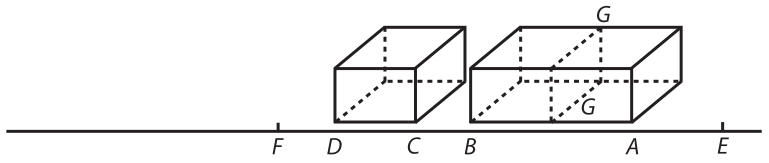
\includegraphics[width=0.84\textwidth]{images/lh03703_162r-d1.pdf}\\
\centering[\textit{Fig. 1}]
\pend
\newpage
\pstart
\begin{center}
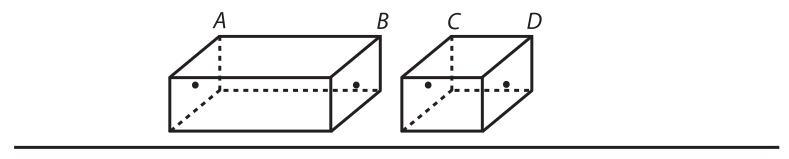
\includegraphics[width=0.84\textwidth]{images/lh03703_162r-d2.pdf}\\
\rule[0pt]{0pt}{0pt}[\textit{Fig. 2}]
\end{center}
\pend
\vspace{1.5em}
\pstart
\begin{center}
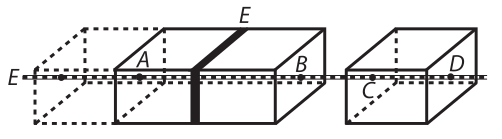
\includegraphics[width=0.57\textwidth]{images/lh03703_162r-d3.pdf}\\
\rule[0pt]{0pt}{0pt}[\textit{Fig. 3}]
\end{center}
\pend
\vspace{1.5em}
\pstart \centering Demonstratio. \setline{1}
\pend 
\vspace{0.5em} 
\pstart \noindent Ponamus \setline{2}si fieri potest, referre quanta sit longitudo corporis \edtext{impellentis, ac}{\lemma{}\Bfootnote{impellentis, \textbar\ id fieri necesse est, quia impulsum\protect\index{Sachverzeichnis}{impulsum} a corpore longiore, \textit{gestr.} \textbar\ ac proinde \textit{L}}} proinde si duo corpora aequivelocia\protect\index{Sachverzeichnis}{corpora aequivelocia}, longitudine inaequalia sibi directe occurrant, \edtext{abripi minus a}{\lemma{abripi}\Bfootnote{\textit{(1)} majus a \textit{(2)} minus a \textit{L}}} majore: id fieri necesse est, quia pars longioris \edtext{$BG$}{\lemma{}\Bfootnote{$BG$ \textit{erg. L}}} \edtext{aequalis toti}{\lemma{aequalis}\Bfootnote{\textit{(1)} \textbar\ est \textit{erg.} \textbar\ part \textit{(2)} toti \textit{L}}} breviori \edtext{$DC$}{\lemma{$DC$}\Bfootnote{\textit{erg. L}}}, tantundem agit, ac proinde residuum \edtext{$GA$}{\lemma{$GA$}\Bfootnote{\textit{erg. L}}}, aliquid praeterea. Totus ergo conatus impressus\protect\index{Sachverzeichnis}{conatus impressus} est aggregatum conatuum singulorum\protect\index{Sachverzeichnis}{aggregatum conatuum singulorum} a singulis partibus impressorum, seu si corpus alterum, altero sit longius duplo, conatus\protect\index{Sachverzeichnis}{conatus} erit duplus, ac proinde \edtext{corpus dimidio minus abripietur a duplo majore}{\lemma{corpus}\Bfootnote{\textit{(1)} minus abripietur a ma \textit{(2)} dimidio [...]
majore \textit{L}}} celerius moto, celeritate dimidia. Haec sane ex illa hypothesi consequuntur.
\pend 
\pstart Si \edtext{duo corpora}{\lemma{duo}\Bfootnote{\textit{(1)} sint \textit{(2)} corpora \textit{L}}} cylindrica\protect\index{Sachverzeichnis}{corpora cylindrica}, basium \edtext{seu latitudinum}{\lemma{}\Bfootnote{seu latitudinum \textit{erg. L}}} aequalium, alterum $AB$ longitudine duplum alterius \edtext{$CD$ sibi}{\lemma{$CD$}\Bfootnote{\textit{(1)} eaque \textit{(2)} sibi \textit{L}}} \edtext{directe}{\lemma{directe}\Bfootnote{\textit{erg. L}}} occurrant aequali velocitate in linea per centra basium, vel \edtext{axes corporum}{\lemma{axes}\Bfootnote{\textit{(1)} eorum \textit{(2)} corporum \textit{L}}} transeunte, quaeritur an corpus majus abrepturum sit secum minus? 
\pend 
\pstart Ponatur id fieri, erit alia quaestio, continueturne motus eadem qua prius celeritate, an non. Et ajo celeritatem ex illo conflictu\protect\index{Sachverzeichnis}{conflictus} diminui debere : nam si manet eadem celeritas\protect\index{Sachverzeichnis}{celeritas}, idem semper sequetur effectus, sive corpus abreptum sit valde exiguum, sive sit mediocre, quod est contra hypothesin, ita enim sequetur nihil quoque referre sive corpus abripiens sit magnum sive sit parvum, nam si longitudo est efficax\protect\index{Sachverzeichnis}{efficax}, erit in utroque; necesse est ergo celeritatem diminui illo conflictu\protect\index{Sachverzeichnis}{conflictus}, sed hic rursus quaerendum est, in qua ratione : necesse est diminui in ea ratione quae est longitudinum, cum caetera omnia sint paria, nec nisi longitudinum ratio habeatur, necesse est ergo eam esse differentiam celeritatum\protect\index{Sachverzeichnis}{differentia celeritatum} ante conflictum\protect\index{Sachverzeichnis}{conflictus} et post conflictum\protect\index{Sachverzeichnis}{conflictus}, quae est longitudinum; et cum in casu praesenti brevius sit longioris dimidium, celeritatem quoque post conflictum\protect\index{Sachverzeichnis}{conflictus} dimidiam esse prioris. Hinc alia \edtext{sequitur propositio}{\lemma{sequitur}\Bfootnote{\textit{(1)} consequentia \textit{(2)} propositio \textit{L}}}, longitudinem esse causam celeritatis,
\edtext{seu, si quid modo a longiore, modo a breviore impellatur, etiamsi longius}{\lemma{seu,}\Bfootnote{\textit{(1)} quod a longiore impellitur, id celerius moveri, etsi impellens ipsum \textit{(2)} si quid [...] impellatur, \textit{(a)} id fortius im \textit{(b)} etiamsi longius \textit{L}}} et brevius aequivelocia\protect\index{Sachverzeichnis}{aequivelocia} supponantur, celerius tamen moveri, quod a longiore impulsum\protect\index{Sachverzeichnis}{impulsum} est. Nam si in casu concursus\protect\index{Sachverzeichnis}{concursus} longius suppositum fuisset non duplum, sed triplum, \edtext{brevioris, brevius}{\lemma{brevioris,}\Bfootnote{\textit{(1)} abreptum \textit{(2)} brevius \textit{L}}} post concursum\protect\index{Sachverzeichnis}{concursus} motum fuisset, differentia eadem celeritatum\protect\index{Sachverzeichnis}{differentia celeritatum}, quae est longitudinum, ac proinde non dimidia sed duabus tertiis celeritatis prioris. 
\pend
\pstart%
Hinc porro sequitur corpus aliquod \edtext{cylindricum motum,}{\lemma{cylindricum}\Bfootnote{\textit{(1)} in \textit{streicht Hrsg.} \textit{(2)} si in vacuo\protect\index{Sachverzeichnis}{vacuum} motum supponatur, \textit{(3)} motum, \textit{L}}} dissolvi in partes infinitas, seu indivisibilia. Quod est absurdum.
\pend 
\pstart Consequentia probatur. Corpus quod a longiore impellitur, movetur celerius quam quod a tardiore, ergo quaelibet portio \edtext{cylindrica}{\lemma{cylindrica}\Bfootnote{\textit{erg. L}}} corporis cylindrici, \edtext{movebitur; anterior, movebitur celerius}{\lemma{movebitur;}\Bfootnote{\textit{(1)} celerius \textit{(2)} anterior, movebitur celerius \textit{L}}} quam quaelibet posterior, ergo eam deseret, cumque portiones assumi possint quantulaecunque, dissolvetur corpus in portiones qualibet dabili minores.
\pend
\count\Afootins=1200
\count\Bfootins=1200
\count\Cfootins=1200
\pstart%
% \centering%
\edtext{Q.E.[D].}{\lemma{A}\Bfootnote{\textit{L ändert Hrsg.}}}
[163~v\textsuperscript{o}]
\pend%